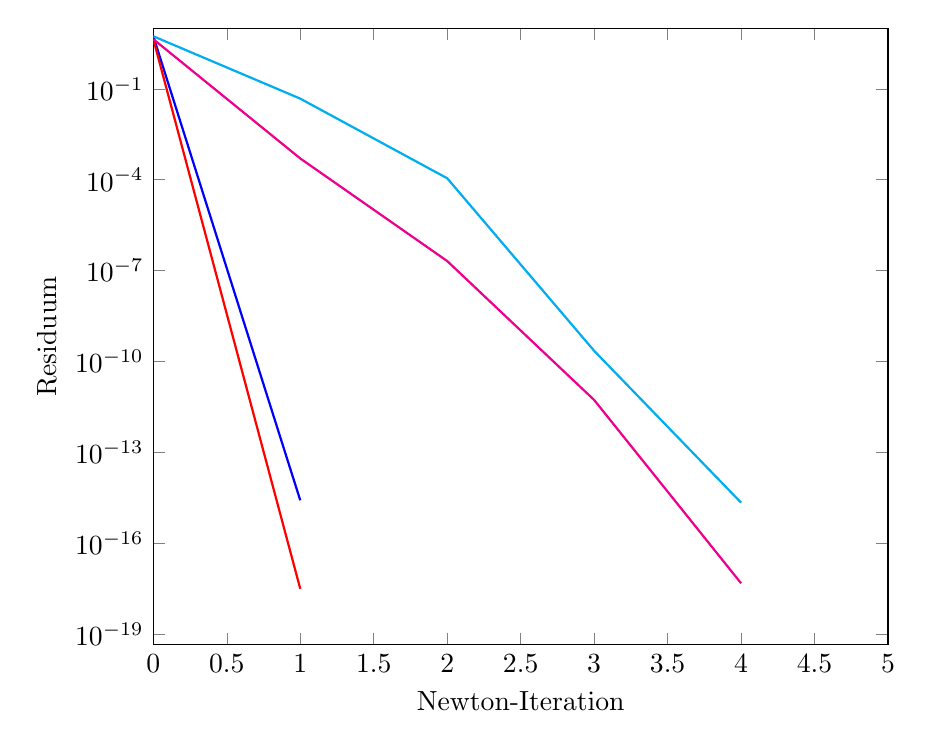
\begin{tikzpicture}[every plot/.append style={thick}] 
\begin{axis}[ 
label style={font=\normalsize}, 
xlabel={Newton-Iteration}, 
ylabel={Residuum}, 
xmin=0, xmax=5, 
ymode=log, 
ymin=0, ymax=10, 
width=0.9\textwidth, 
grid style=dashed, 
] 
\addplot[ 
color=blue, 
] 
coordinates { 
(0, 5.44e+00)(1, 2.66e-15)}; 
\addplot[ 
color=red, 
] 
coordinates { 
(0, 4.35e+00)(1, 3.20e-18)}; 
\addplot[ 
color=cyan, 
] 
coordinates { 
(0, 5.43e+00)(1, 4.75e-02)(2, 1.12e-04)(3, 2.27e-10)(4, 2.22e-15)}; 
\addplot[ 
color=magenta, 
] 
coordinates { 
(0, 4.35e+00)(1, 5.05e-04)(2, 2.08e-07)(3, 5.42e-12)(4, 4.86e-18)}; 
\end{axis} 
\end{tikzpicture} 
